\section{Problema 1}
\begin{frame}{Contenido}
        \tableofcontents[sections={2}]
\end{frame}

\subsection[Presentacion]{Presentación del problema}
\begin{frame}{Presentación del problema}
    \begin{columns}
        \begin{column}{0.47\textwidth}
            Sea la catenaria:
            \begin{figure}[h]
                \includegraphics[width=5cm]{Imagenes/Catenaria.png}
                \centering
            \end{figure}
        \end{column}
        \begin{column}{0.47\textwidth}
                Cuya fórmula es:                
                \[y=C_{1}*\cosh(\frac{x+C_{2}}{C_{1}})\]
                y cuyas condiciones de extremo son:
                \[x_{1}=-1.5 \]
                \[y_{1}=2 \]
                y:
                \[x_{2}=1.5 \]
                \[y_{2}=3 \]             
        \end{column}
    \end{columns}
\end{frame}
\begin{frame}{Operaciones iniciales}
    \centering
    Para el cálculo de $c_{2}$ tendríamos:                
                \[C_{2}=C_{1}*\acosh(\frac{y}{C_{1}})-x\]
    Reemplazamos para los valores iniciales del extremo derecho:
    \[C_{2}=C_{1}*\acosh(\frac{y_{2}}{C_{1}})-x_{2}\]
    y luego reemplazamos $c_{2}$ para los valores iniciales del extremo izquierdo:
    \[y_{1}=C_{1}*\cosh(\frac{x+(C_{1}*\acosh(\frac{y_{2}}{C_{1}})-x_{2})}{C_{1}})\]
\end{frame}

\begin{frame}{Gráfica de la ecuación $y(c_{1})$}
    \centering
    \begin{tikzpicture}[samples=100]
        \begin{axis}[
            xmin=0.5,xmax=2.5,
            ymin=1,ymax=3]
            \addplot[domain=0.5:2.5,draw=red,ultra thick]
        {(\x)*cosh((-1.5+(\x*acosh((3)/(\x))-1.5))/(\x))};           \addplot[domain=0:3,draw=blue]{2};
        \end{axis}       
    \end{tikzpicture}
\end{frame}
\subsection[R. iteraciones]{Resolución por iteraciones sucesivas}
\begin{frame}[fragile,allowframebreaks]{Resolución del problema en Python por iteraciones sucesivas}

    Declaramos variables del programa y el error admisible:
\begin{lstlisting}[language=Python]
    #@title Variables iniciales:
    import math
    #Se pide la cantidad 
    #de decimales admisibles
    n1=5 #@param {type:"integer"}
    #se calcula el error
    err_admisible=10**(-n1)
\end{lstlisting}
\framebreak
Declaramos las condiciones de extremo del problema y los límites entre los que buscará una respuesta:
\begin{lstlisting}[language=Python]
    x1=-1.5 #@param {type:"number"}
    y1=2 #@param {type:"number"}
    x2=1.5 #@param {type:"number"}
    y2=3 #@param {type:"number"}
    li=0.75 #@param {type:"number"}
    lf=3 #@param {type:"number"}
\end{lstlisting}
\framebreak
Se calcula los valores de y1 para el límite superior e inferior escogido de c1
\begin{lstlisting}[language=Python]
    c2i=li*math.acosh(y2/li)-x2
    y1i=li*math.cosh((x1+c2i)/(li))
    c2f=lf*math.acosh(y2/lf)-x2
    y1f=lf*math.cosh((x1+lf)/(lf))
\end{lstlisting}
\framebreak

Calculamos el valor intermedio de y1 considerando el valor medio de c1:
\begin{lstlisting}[language=Python]    
    c1a=(li+lf)/2
    c2b=c1a*math.acosh(y2/c1a)-x2
    y1b=c1a*math.cosh((x1+c2b)/(c1a))
\end{lstlisting}
\framebreak
si el límite inicial es mayor que el límite final ejecutamos este código,
\begin{lstlisting}[language=Python]         
    if y1i>y1f:
      while abs(y1-y1b)>err_admisible:
        if y1b>y1:
            li=c1a
        else:
            lf=c1a
        c1a=(li+lf)/2
        c2b=c1a*math.acosh(y2/c1a)-x2
        y1b=c1a*math.cosh((x1+c2b)/(c1a))
\end{lstlisting}
el proceso termina cuando la diferencia de y1 y y1b es menor al error admisible\\
\framebreak
si el límite inicial es menor que el límite final ejecutamos este código
\begin{lstlisting}[language=Python]             
    else:
      while abs(y1-y1b)>err_admisible:
        if y1b>y1:
            lf=c1a
        else:
            li=c1a
        c1a=(li+lf)/2
        c2b=c1a*math.acosh(y2/c1a)-x2
        y1b=c1a*math.cosh((x1+c2b)/(c1a))
\end{lstlisting}
el proceso termina cuando la diferencia de y1 y y1b es menor al error admisible\\
\framebreak
se imprimen los resultados:
\begin{lstlisting}[language=Python]   
        print("y1a: ",y1a)
        print("y2a: ",y2a)
        print("C1a=", c1a)
        print("C2b=",c2b)
\end{lstlisting}
   
\end{frame}
\begin{frame}{Resultados del proceso}
            Resultados obtenidos:
            \begin{figure}[h]
                \includegraphics[width=6cm]{Imagenes/Resultados1.png}
                \centering
            \end{figure}
\end{frame}
\begin{frame}{Explicación gráfica del proceso I}
\centering
    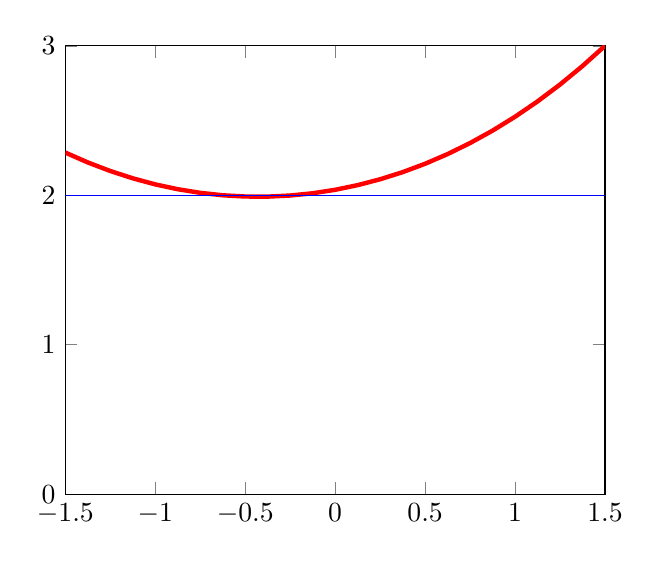
\begin{tikzpicture}
        \begin{axis}[
            xmin=-1.5,xmax=1.5,
            ymin=0,ymax=3]
            \addplot[domain=-1.5:1.5,draw=red,ultra thick]{1.99*cosh(((\x)+0.4285)/1.99)};           \addplot[domain=-1.5:1.5,draw=blue]{2};
        \end{axis}       
    \end{tikzpicture}
\end{frame}
\begin{frame}{Explicación gráfica del proceso II}
\centering
    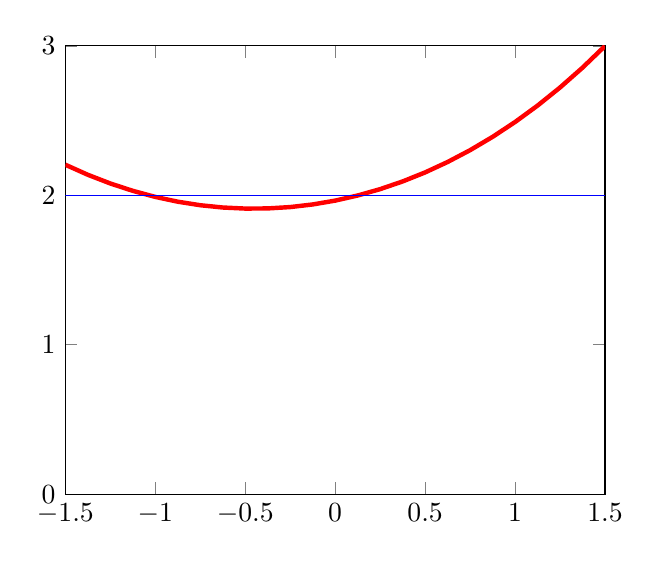
\begin{tikzpicture}
        \begin{axis}[
            xmin=-1.5,xmax=1.5,
            ymin=0,ymax=3]
            \addplot[domain=-1.5:1.5,draw=red,ultra thick]{1.91*cosh(((\x)+0.453)/1.91)};           \addplot[domain=-1.5:1.5,draw=blue]{2};
        \end{axis}       
    \end{tikzpicture}
\end{frame}
\begin{frame}{Explicación gráfica del proceso III}
\centering
    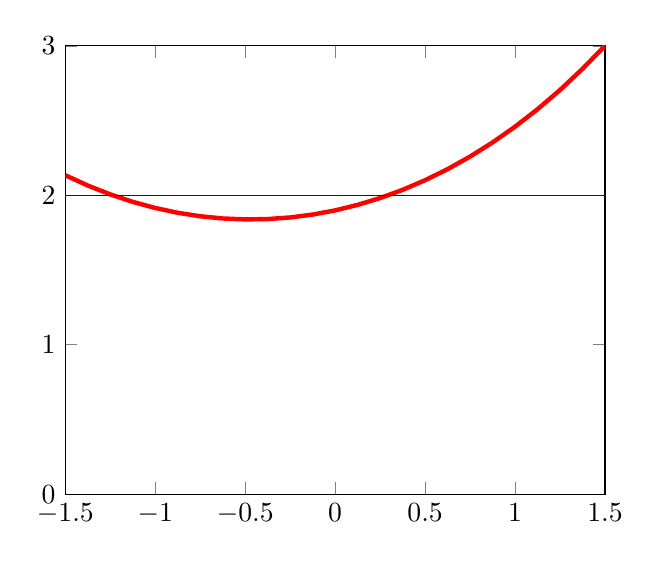
\begin{tikzpicture}
        \begin{axis}[
            xmin=-1.5,xmax=1.5,
            ymin=0,ymax=3]
            \addplot[domain=-1.5:1.5,draw=red,ultra thick]{1.838*cosh(((\x)+0.471)/1.838)};           \addplot[domain=-1.5:1.5,draw=blue]{2};
        \end{axis}       
    \end{tikzpicture}
\end{frame}
\begin{frame}{Explicación gráfica del proceso IV}
\centering
    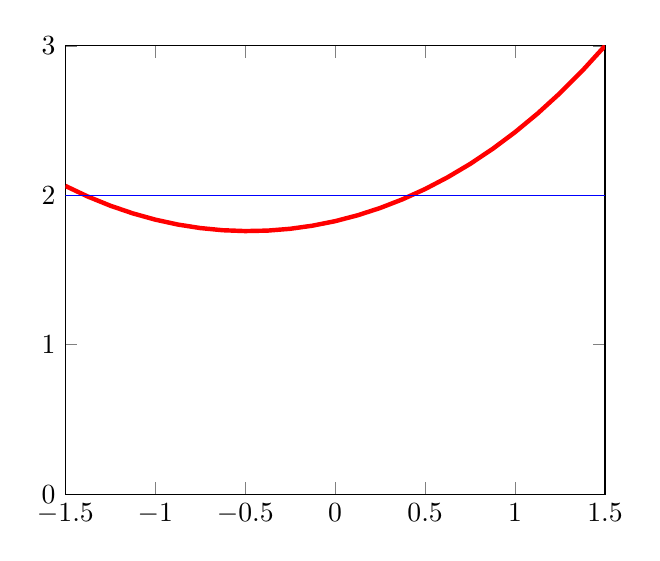
\begin{tikzpicture}
        \begin{axis}[
            xmin=-1.5,xmax=1.5,
            ymin=0,ymax=3]
            \addplot[domain=-1.5:1.5,draw=red,ultra thick]{1.76*cosh(((\x)+0.4824)/1.76)};           \addplot[domain=-1.5:1.5,draw=blue]{2};
        \end{axis}       
    \end{tikzpicture}
\end{frame}
\begin{frame}{Explicación gráfica del proceso V}
\centering
    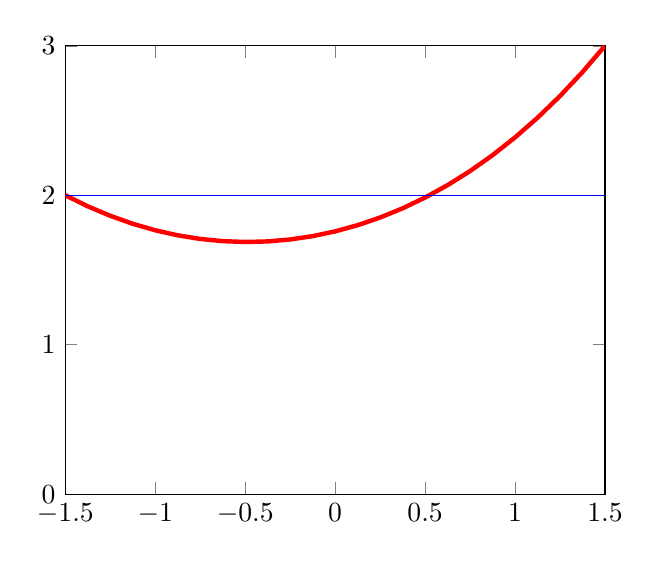
\begin{tikzpicture}
        \begin{axis}[
            xmin=-1.5,xmax=1.5,
            ymin=0,ymax=3]
            \addplot[domain=-1.5:1.5,draw=red,ultra thick]{1.6871*cosh(((\x)+0.4878)/1.6871)};           \addplot[domain=-1.5:1.5,draw=blue]{2};
        \end{axis}       
    \end{tikzpicture}
\end{frame}
  
\subsection[R. analitica]{Resolución analítica}
\begin{frame}[fragile,allowframebreaks]{Resolución analítica}
    \textbf{Cálculo de las constantes de una catenaria.-}  Las constantes $\mu, c_{1}, c_{2}$, para unas condiciones iniciales dadas, no pueden calcularse más que mediante técnicas de análisis numérico.\footcite{Car12}
    Esto debido a que las ecuaciones con funciones trascendentes que tienen a una variable por dentro y por fuera de la función trascendente no pueden resolverse por métodos analíticos. \\Para terminar de resolver la catenaria, utilizaremos el siguiente enlace con el código expuesto hecho en Google Coolab: \href{https://colab.research.google.com/drive/1zJW8x3nobNhw7CngeY5IqShL2OD_w9AH?hl=es#scrollTo=KHneYamBqSlN}{Enlace de Coolab}
    
    
\end{frame}


\subsection[Grafica]{Gráfica de la ecuación}
\begin{frame}{Gráfica de cuerda corta}
\centering
    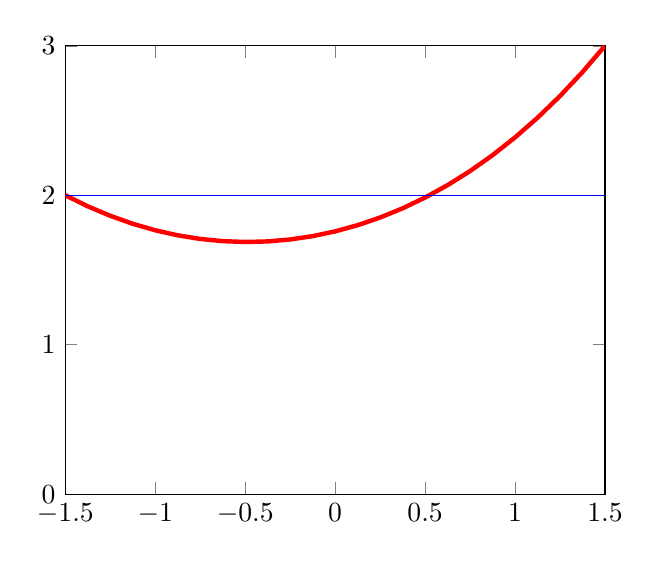
\begin{tikzpicture}
        \begin{axis}[
            xmin=-1.5,xmax=1.5,
            ymin=0,ymax=3]
            \addplot[domain=-1.5:1.5,draw=red,ultra thick]{1.6871*cosh(((\x)+0.4878)/1.6871)};           \addplot[domain=-1.5:1.5,draw=blue]{2};
        \end{axis}       
    \end{tikzpicture}
\end{frame}
\begin{frame}{Gráfica de cuerda larga}
\centering
    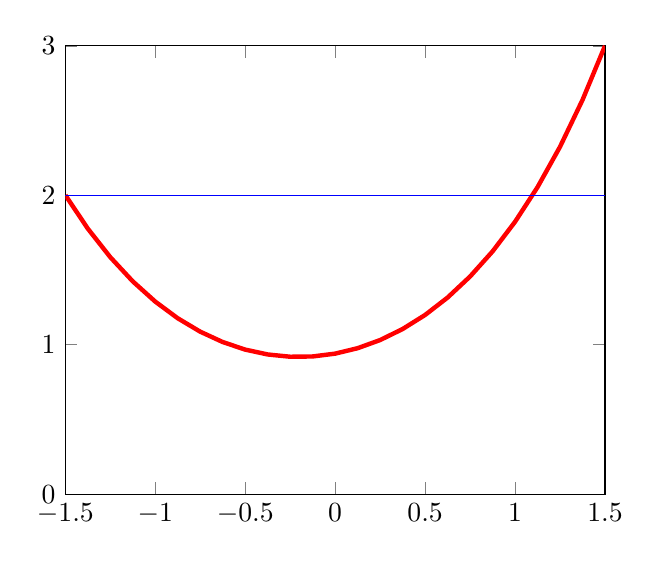
\begin{tikzpicture}
        \begin{axis}[
            xmin=-1.5,xmax=1.5,
            ymin=0,ymax=3]
            \addplot[domain=-1.5:1.5,draw=red,ultra thick]{0.91796875*cosh(((\x)+0.20106)/0.91796875)};           \addplot[domain=-1.5:1.5,draw=blue]{2};
        \end{axis}       
    \end{tikzpicture}
\end{frame}

\subsection[Importancia]{Importancia de la catenaria}

\begin{frame}[fragile,allowframebreaks]{Importancia de la catenaria}
    El cable es un elemento flexible que, sujeto a cargas externas, adquiere una forma concreta llamada funicular, que depende de la magnitud y la posición de las mismas, la forma que adopta el cable al estar sujeto en sus extremos y expuesto a la acción de su propio peso es justamente la catenaria.
\begin{figure}[h]            \includegraphics[width=10cm]{Imagenes/FormasCat.jpg}
    \caption{Formas que adoptan los cables al estar someditos a diferentes cargas.}
    \centering
\end{figure}

\framebreak
Las estructuras atirantadas se han utilizado extensamente a lo largo de la historia, hay muchos ejemplos de puentes colgantes con materiales tipo bambú, cañas o cuerdas. Más actualmente se han construido un gran número de edificios con estructuras de cables, siendo el acero galvanizado y el acero inoxidables los materiales más usados actualmente.
      \begin{figure}[h]
        \includegraphics[width=10cm]{Imagenes/UnionesCat.jpg}
        \caption{Uniones de Cables.}
                \centering
            \end{figure}

\framebreak
Entre las estructuras que utilizan a los cables, o se sirven de la forma de la catenaria, podemos encontrar los siguientes grupos
\begin{itemize}
    \item Estructuras soportadas por cables
    \item Estructuras superficiales formadas por cables.
    \item Estructuras con arcos catenarios como columnas de apoyo.
\end{itemize}
\framebreak
\textbf{Estructuras  soportadas por cables:}
\\Se caracterizan porque los cables trabajan individualmente, como elementos suspendidos o como columnas a tracción, para soportar elementos estructurales como vigas, superficies o edificios.
    \begin{figure}[h]
       \includegraphics[width=10cm]{Imagenes/Mill Lon.jpg}
            \centering
            \caption{Millenium Bridge, Londres.}
    \end{figure}

\framebreak
Un ejemplo de edificio soportado por cables es el banco de la reserva federal de Mineapolis, de Gunnar Birkerts (1973) en el que de dos cables anclados a dos núcleos de hormigón separados 100 m cuelgan 11 plantas.
    \begin{figure}[h]
       \includegraphics[width=5cm]{Imagenes/BancoR.jpg}
                \centering
                \caption{Banco de la reserva federal, Mineapolis}
    \end{figure}

\framebreak
\textbf{Estructuras  superficiales formadas por cables:}
\\Se caracterizan porque los cables trabajan conjuntamente formando estructuras superficiales o incluso bidimensionales.
\\Se utilizan fundamentalmente para cubiertas y, en ellas, los cables se disponen paralelamente o de forma radial, llegando a cubrir luces de entre 45 m y 135 m\footcite{Lui15}
    \begin{figure}[h]
       \includegraphics[width=10cm]{Imagenes/Aeroupuerto.jpg}
                \centering
                \caption{Terminal del aeropuerto de Dulles}
    \end{figure}

\framebreak
\textbf{Estructuras  con arcos catenarios:}
\\Antoni Gaudí, arquitecto español de mediados del s. XIX, trabajó un sistema estructural basado en la mecánica y la geometría de las curvas funiculares, a partir de la observación de formas orgánicas en la naturaleza.
    \begin{figure}[h]
       \includegraphics[width=6cm]{Imagenes/ArcosCate.jpg}
       \caption{Arcos catenarios de Gaudi}
                \centering
    \end{figure}

     
\end{frame}

\begin{frame}[fragile,allowframebreaks]{Aproximacion a la catenaria por los metodos de energia}
    Mencionaremos, por último, que el problema de la catenaria puede abordarse desde un punto de vista completamente distinto, partiendo del hecho de que la catenaria debe ser la curva que une dos puntos con una longitud dad con la mínima energía potencial. La energía potencial de una curva es:\footcite{Car12}
\[E(y)= \int_{0}^{L} gy(s)\rho \cdot ds=\rho g \int_{x_{0}}^{x_{1}} y(x) \sqrt{1+y^{'}(x)^{2}} \cdot dx\]
de donde obtenemos que:
\[y=\frac{h}{2}+\frac{a}{\gamma}(\cosh(\gamma \frac{x}{a} +C_{2})-\cosh(C_{2})\cosh(\gamma) )\]
siendo los puntos extremos de la catenaria $(-a,0)$ y $(a,h)$


     
\end{frame}
